\documentclass[cnatzke_thesis_proposal.tex]{subfiles}
\begin{document}

\chapter{The GRIFFIN Spectrometer at TRIUMF}

%%%%%%%%%%%%%%%%%%%%
\subsection{TRIUMF Rare Isotope Beam Facility}
%%%%%%%%%%%%%%%%%%%%
\begin{figure}[H]
  \begin{center}
    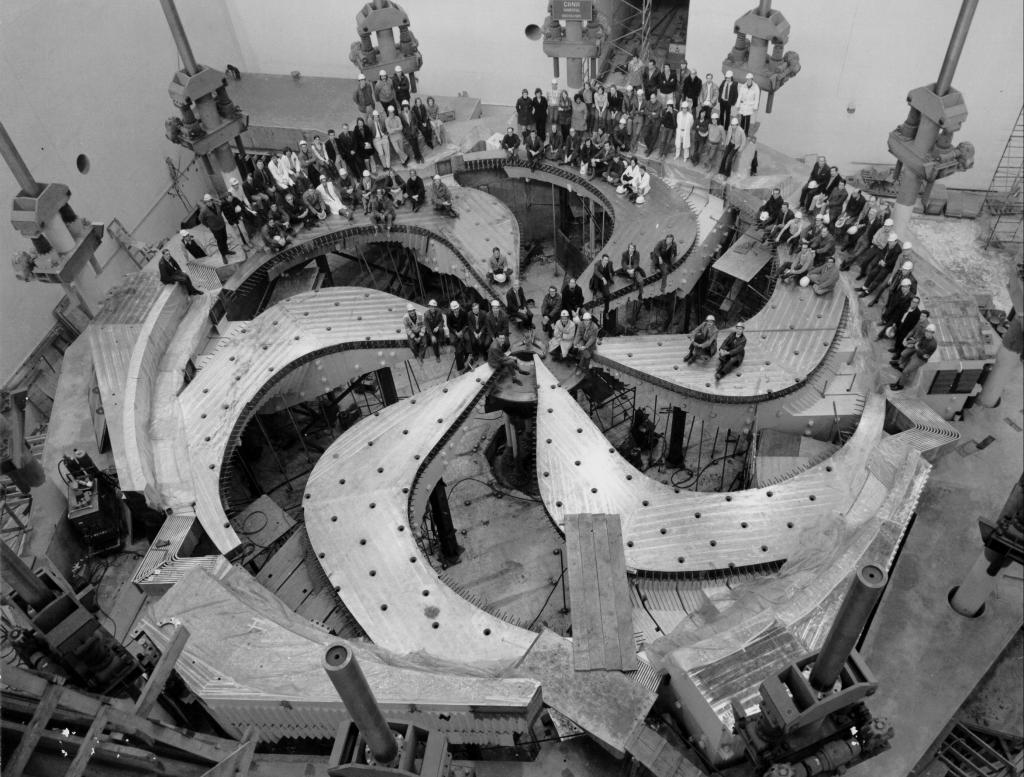
\includegraphics[scale=.15]{triumf_cyclotron_construction_1972.jpg}
  \end{center}
  \caption{TRIUMF cyclotron during initial construction (1972) - Figure courtesy of TRIUMF.}
  \label{fig:triumf_cyclotron_1972}
\end{figure}

The proposed experiment will be performed at TRIUMF located in Vancouver, British Columbia. TRIUMF 


The TRIUMF-ISAC experimental facility located in Vancouver, BC, Canada was initially designed by Richardson in 1962 and later built and commissioned in Canada with the first beam extraction taking place in 1974 \cite{Bylinskii2014}. The Rare Isotope Beam (RIB) facility specializes in producing exotic nuclei via a 500 MeV $H^{-}$ cyclotron that produces high intensity proton beams up to 100 $\mu A$.  This Isotope separation online (ISOL) facility directs a $p^+$ beam at a thick target that then undergoes nuclear reactions including spallation, fragmentation, and induced fission \cite{Bricault2014}.  To determine a specific isotope yield for this process see Eq.\ref{eq:isol_yeild} where $\sigma_P$ is the proton beam intensity hitting the target, $\sigma(A, Z)$ is the cross section of the production of the specified isotope and $N_T$ is the number of target nuclei per $cm^2$, the efficiencies for $\epsilon_{Dif}$ is diffusion, $\epsilon_{Eff}$ effusion,  $\epsilon_{Ion}$ ionization, and $\epsilon_{Trans}$ beam transport \cite{Bricault2014}.

\begin{equation}
  \Phi(A,Z) = \phi_P \sigma(A,Z) N_T \epsilon_{Dif} \epsilon_{Eff} \epsilon_{Ion} \epsilon_{Trans}
  \label{eq:isol_yeild}
\end{equation}

These reactions generate a variety of short lived nuclei that are subsequently mass separated and delivered to the experiment halls, see \ref{fig:ISAC_HALL} \cite{Dombsky2014}.

These thick targets are available in several different materials depending on the type of exotic nuclei that is needed, typical target materials are Si, Ti, Nb, Zr, Ta, and U \cite{Dilling2014}.  The targets are operated at high temperatures (2300 $^{\circ}$C) in order to enhance diffusion and effusion of the product nuclei \cite{Dombsky2014}.

\begin{center}
\begin{figure}[H]
  \begin{center}
    \includegraphics[scale=.18]{isac_i_facility.png}
  \end{center}
  \caption{Schematic view of the TRIUMF-ISAC facility \cite{Dilling2014}}
  \label{fig:ISAC_HALL}
\end{figure}
\end{center}

% for IGLIS Raeder2014
% Talk about IGLIS probably...

\subsection{TITAN - TRIUMF's Ion Trap From Atomic and Nuclear Science \cite{Dilling2006}}

\begin{figure}[H]
  \begin{center}
    \includegraphics[scale=.5]{TITANsetup.pdf}
  \end{center}
  \caption{Schematic view of TITAN trap beamline, courtesy of TRIUMF \& TITAN group}
  \label{fig:titan_beamline}
\end{figure}

The TITAN groups' experimental setup consists of 5 traps, Cooler Penning Trap (CPET), Measurement Penning Trap (MPET), Multi-reflection Time of Flight Mass Spectrometer (MR-TOF-MS), Electron Beam Ion Trap (EBIT) as well as a Radio Frequency Quadapole (RFQ) linear Paul trap which functions as a cooler and buncher.  These systems can operate alone or in conjunction such as where the RFQ cools and bunches the beam before passing it off to the MR-TOF-MS.  From there the MR-TOF-MS can clean the beam for a specific mass to great precision before passing it off to the EBIT for further charge breeding and possible injection into MPET or CPET.  The ability for TITAN to combine instruments for purification and trapping gives it a unique ability to probe fundamental nuclear and atomic properties.

\subsection{The TITAN Electron-Beam Ion Trap (EBIT)}

\begin{figure}[H]
  \begin{center}
    \includegraphics[scale=.3]{EBIT1.png}
  \end{center}
  \caption{Schematic view of EBIT}
  \label{fig:EBIT_CUTOUT}
\end{figure}

The electron-beam ion trap serves to generate highly-charged ions (HCIs) by means of an intense electron beam causing electron-impact ionization and trap them via electro-magnetic fields.  The TITAN EBIT was built at the Max-Planck-Institute for Nuclear Physics (MPI-K) in Heidelberg from 2004-2006 \cite{TITAN_EBIT_2010}.  The EBIT uses a very strong (near 6T) magnetic field generated by pair of coils in a Helmholtz geometry to compress the electron beam creating a very high current density to facilitate the electron-impact ionization.  The HCIs are trapped in the axial direction by a symmetric electrostatic quadrupole potential well which is achieved via applying a potential to the EBIT's drift tubes.  Radial confinement is handled by the electron-beam space-charge potential along with the previously mentioned strong magnetic field \cite{TITAN_EBIT_2010}.

\begin{figure}[H]
  \begin{center}
    \includegraphics[scale=.3]{ebit_schematic.png}
  \end{center}
  \caption{Schematic view of EBIT \cite{PALFFY_THESIS}}
  \label{fig:schematic_ebit}
\end{figure}

(Fig. \ref{fig:schematic_ebit} )
**DESCRIBE  THRESHOLD CHARGE BREEDING**
For a Penning trap the relative precision of the mass measurement is proportional to the charge state of the ion which can be approximated via (Eq. \ref{eq:ebit_resolving_power} \cite{TITAN_EBIT_2010})


\begin{equation}
  \frac{\delta m}{m} \propto \frac{m}{qB} \frac{1}{T_{RF}} \frac{1}{\sqrt{N}}
  \label{eq:ebit_resolving_power}
\end{equation}

here $T_{RF}$ represents the excitation time in the magnetic field $B$ with $N$ representing the number of measurements.  From this it is clear the powerful benefits inherent in using an EBIT to further charge breed ions before passing them to a Penning trap \cite{TITAN_EBIT_2010}.

The time to breed to a specific charge state is given by (Eq. \ref{eq:ebit_stripping_time})
\begin{equation}
  \tau_{i}(q) = \sum_{q'=0}^{q-1}\langle n_e v_e \sigma^{I}_{q', q'+1} \rangle^{-1}
  \label{eq:ebit_stripping_time}
\end{equation}

where $\sigma^{I}_{q', q'+1}$ is the cross section for single ionization and $n_e v_e$ is equal to the current density divided by the elementary charge $\frac{j_e}{e}$ \cite{SPRINGER_1997}.


\end{document}
